% !TEX root =  paper.tex

\section{Approach}
\label{sec:approach}

Our approach for driving web app state exploration consists of two parts, namely, 
(1) a method for identifying actionables
using the web elements' structural and visual style features; and 
(2) a mechanism for ranking which events to fire
while exploring the states,  in order to to achieve a higher coverage.
In the following subsections,
we provide the details of these two steps.

\subsection{Predicting actionables}
\label{subsec:identifying-elements}
Our approach to identifying actionables
is based on a simple but novel intuition:
usually, when a user looks at a web page,
they are able to intuit where to click or
how to interact with the page based on what elements look like.
Styling actionables so that they look distinguishing
on the web page
is a recommended usability practice~\cite{w3c-actionable-elements, bbc-actionables-usability-tips}.
A clickable element, for example, might have an underlined text,
a border, or a shadow,
or might look like a button.
The intuition for our approach is that such stylistic
features can be used to train a machine learning model
to predict which elements on the page are actionable.

\Cref{fig:model-training-pipeline} depicts our overall pipeline for learning.
We explain the details of our learning process in the following subsections.

\begin{figure}
	\centering
	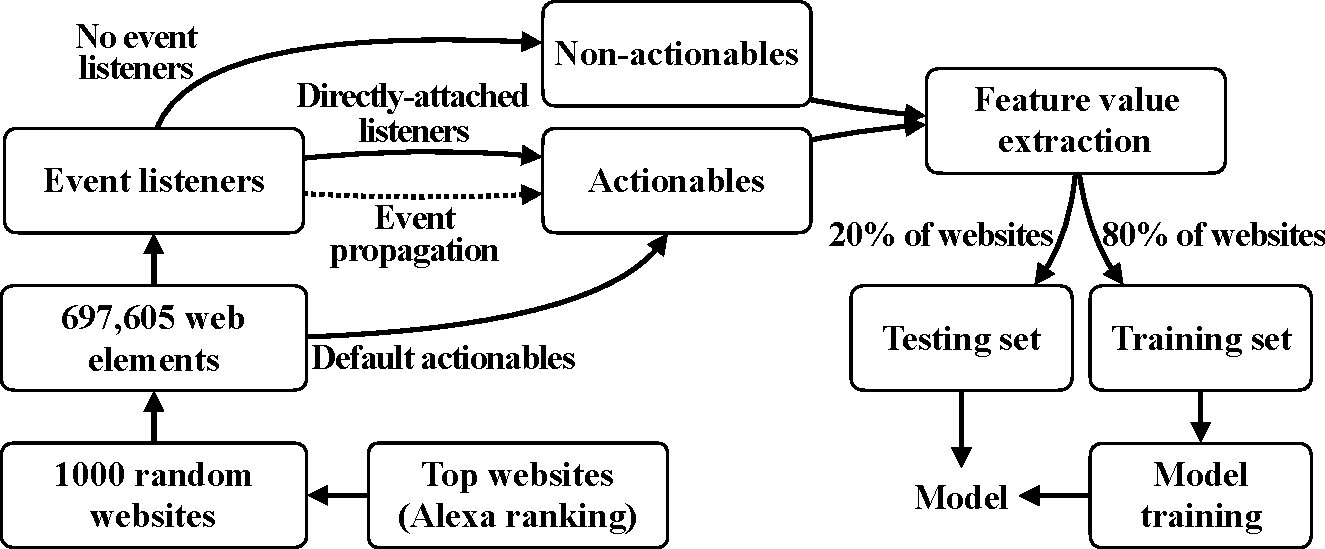
\includegraphics[width=\linewidth]{figures/training-pipleline}
	\caption{Our machine learning model training pipeline.}
	\label{fig:model-training-pipeline}
\end{figure}

\header{Data collection for training}
To collect data for training a model, 
we need a large set of pre-identified (1)  actionable elements to be used 
as positive examples, and (2) elements without any event listeners to be used as negative examples.

We collect these elements by crawling a large set of web apps in the wild.
To that end, we developed a script to randomly choose 1,000 websites
from Alexa's top ranking list of URLs~\cite{alexa-ranking}.
The reason for this random selection is 
to cover a wide range of sites 
that have been developed with different front-end frameworks, libraries, and development styles.

The script subsequently loads each URL in the Chrome web browser, 
traverses the DOM loaded in the web browser,
and collects all the \html elements present in the web page.
For each element, the script collects any attached event listeners.
The event listeners are retrieved using Chrome DevTools~\cite{chrome-dev-tools},
which have direct access to the browser's internal engine,
and thus is accurate. Note that this access is only needed for collecting the training data. %and does not affect websites' execution.

If an element has an attached event listener,
it is considered \emph{actionable} and is stored for
later analysis along with the type of the event(s) handled.
In addition, we consider \html elements which are \textit{actionable by default}, 
such as hyperlinks and buttons, as positive examples, regardless if whether they have a \js event listener.
The reason for this is that these elements can change the state even without
an explicitly attached \js event.

\begin{figure}%[b]
	\centering
	\begin{subfigure}[b]{0.32\linewidth}
		\centering
		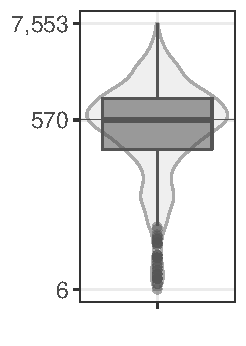
\includegraphics[scale=0.64]{figures/number-of-dom-nodes}
		\caption{\#DOM nodes}
		\label{fig:number-of-dom-nodes}
	\end{subfigure}
	\begin{subfigure}[b]{0.32\linewidth}
		\centering
		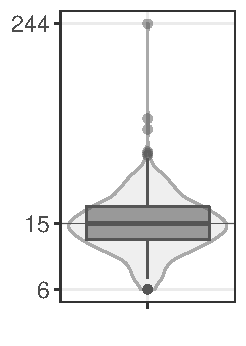
\includegraphics[scale=0.64]{figures/dom-height-distribution}
		\caption{DOM height}
		\label{fig:dom-height-distribution}
	\end{subfigure}
	\begin{subfigure}[b]{0.32\linewidth}
		\centering
		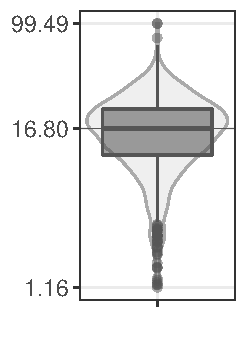
\includegraphics[scale=0.64]{figures/elements-with-event-listeners-percentage}
		\caption{\%Actionables}
		\label{fig:percentage-elements-listeners}
	\end{subfigure}
	\caption{Descriptive statistics for the training websites.}
	\label{fig:websites-info}
\end{figure}

% \header{Characteristics of the collected data}
\Cref{fig:websites-info} depicts violin plots
summarizing the characteristics of the websites 
used in the learning process.
As it can be observed, the websites are quite complex
in terms of the number of DOM elements (\Cref{fig:number-of-dom-nodes})
and the height of the DOM tree (\Cref{fig:dom-height-distribution}).
In addition, we have shown the distribution of the percentage of the actionables
over all the DOM elements existing in each website
in \Cref{fig:percentage-elements-listeners}.
Notice that the median percentage of actionable elements is 16.80\%.
Moreover, we found that 53.26\% of these actionables 
are elements other than the \textit{default actionables} (i.e., hyperlinks and buttons).

\header{Incorporating event propagation}
Firing certain events on DOM elements 
causes the same event to be triggered on the element's ancestors.
% i.e., if there is an event listener attached to those elements,
% normally they will be executed too.
For instance, when a user clicks on a button,
all the button's ancestor elements are also clicked too through event propagation.
The order in which the event listeners of the same type
attached to the ancestor elements
are executed can be different: %determined by the user
i.e., first execute the events attached to the ancestors, going down in the DOM hierarchy---the \textit{capture} phase---%
or first execute the events attached to the element itself, going up in the hierarchy---the \textit{bubble} phase~\cite{event-bubble-capture}.

To incorporate this behavior in the training model,
for the event handlers that bubble,
we mark the descendant elements of an actionable
%(i.e., an element that has an event listener directly attached to it)
to be actionable too.
%This is because firing those events on the descendant elements will eventually fire the event handler
%attached to the top-level element.
In our experience, this can greatly improve the accuracy of the trained models,
because the values for most of the structural and visual styles (i.e., the models' features)
are also \textit{inherited} by the descendant elements, through CSS inheritance~\cite{css-cascade-inheritance}.


\begin{table*}[h]
	\caption{Features used in the trained models}
	\centering
	\footnotesize
	\setlength\tabcolsep{3px}
	\begin{threeparttable}
		\bgroup
		%\def\arraystretch{1.5}
		\begin{tabular}{l p{15.5cm}}
			\toprule
			\textbf{Type} & \textbf{Features} \\ \midrule
			
			\textbf{DOM-related}	& 
				Bounding box position and size (x, y, width, height),
			    DOM depth, 
			    number of descendants,
			    height of the subtree rooted at the element \\ \midrule
			
			\textbf{Visual (\css)} &    
				\smcode{align-content}, 
				\smcode{align-items}, 
				\smcode{align-self}, 
				\smcode{backface-visibility}, 
				\smcode{border-block-end-style}, 
				\smcode{border-block-start-style}, 
				\smcode{border-bottom-style}, 
				\smcode{border-collapse}, 
				\smcode{border-inline-end-style}, 
				\smcode{border-inline-start-style}, 
				\smcode{border-left-style}, 
				\smcode{border-right-style}, 
				\smcode{border-top-style}, 
				\smcode{box-sizing}, 
				\smcode{clear}, 
				\smcode{cursor}, 
				\smcode{display}, 
				\smcode{flex-direction}, 
				\smcode{flex-grow}, 
				\smcode{flex-wrap}, 
				\smcode{float}, 
				\smcode{font-style}, 
				\smcode{font-weight}, 
				\smcode{hyphens}, 
				\smcode{justify-content}, 
				\smcode{list-style-position}, 
				\smcode{list-style-type}, 
				\smcode{mix-blend-mode}, 
				\smcode{object-fit}, 
				\smcode{opacity}, 
				\smcode{outline-style}, 
				\smcode{overflow-wrap}, 
				\smcode{overflow-x}, 
				\smcode{overflow-y}, 
				\smcode{pointer-events}, 
				\smcode{position}, 
				\smcode{resize}, 
				\smcode{table-layout}, 
				\smcode{text-align}, 
				\smcode{text-decoration-line}, 
				\smcode{text-decoration-style}, 
				\smcode{text-overflow}, 
				\smcode{text-rendering}, 
				\smcode{text-size-adjust}, 
				\smcode{text-transform}, 
				%\smcode{touch-action}, 
				\smcode{transform-style}, 
				\smcode{unicode-bidi}, 
				\smcode{user-select}, 
				\smcode{visibility}, 
				\smcode{white-space}, 
				\smcode{word-break} \\
				
			& 
				In addition, binary values determining whether
				a value other than the default value 
				is set 
				for the following \css properties:
				Animation-related properties (i.e., \smcode{animation-name} and \smcode{transition-property}),
			    \smcode{background},
			    \smcode{border} and \smcode{outline} (at any of the four sides of the element),
			    \smcode{box-shadow},
			    \smcode{text-decoration},
			    \smcode{touch-action},
			    \smcode{transform},
			    \smcode{will-change}, and
			    \smcode{z-index}. \\
			\bottomrule
		\end{tabular}
		\egroup
		%\begin{tablenotes}
			%\item[\textdagger] 
		%\end{tablenotes}
	\end{threeparttable}
	\label{table:model-features}
\end{table*}

\header{Training features}
For each element,
we collect and store the values for a set of \totalNumberOfFeatures features
of structural and visual styles,
which will be used as learning features in the trained models.
\Cref{table:model-features} lists these features.
The values for these features are extracted via the DOM API.


There are two sets of such learning features:

\header{(Structural) DOM-related features}
These include:
\begin{itemize}[leftmargin=*]
	\item The absolute position (from the top-left corner of the web browser window)
	and size of the bounding box of the element
	as rendered in the web browser. 
	The rationale behind using the bounding box is that, 
	intuitively, a relatively large element is less probable to have certain event listeners.
	In addition, 
	an element with abnormal positioning (e.g., negative values, which corresponds to an element outside the viewport)
	is less likely to be actionable.
	We use the \code{Element.getBoundingClientRect()} DOM function to retrieve elements' bounding boxes.
	
	\item DOM depth, which corresponds to the depth of the element in the DOM hierarchy.
	The intuition here is that 
	the elements which are closer to the \html root (e.g., have smaller depth)
	are less likely to have event listeners to be actionable by users.
	Rather, they are mostly used in defining the structure of web pages.
	
	\item Number of descendants, and height of the subtree rooted at the element.
	These values determine the \textit{complexity} of the DOM subtree
	under the element.
	It is intuitive that elements which are more complex 
	(e.g., a \code{<nav>} element which is used as a container for menu items)
	are not actionable.
	%Instead, the elements contained in the complex containers are more likely to have event listeners.
\end{itemize}

Note that, in our machine learning models,
we did not include elements' ``tag name'' as a feature.
The reason is that 
any element with any tag name can become actionable;
as a result, in practice we observed that including the tag name does not generally 
improve the trained models.
In addition, it is now possible to define \textit{custom \html elements}
with custom tag names,
both supported natively in all major web browsers in the 
Web Components standard~\cite{web-components},
and also in several popular frameworks (e.g., Angular~\cite{angular-custom-elements}).
In such cases, custom tag names would be unknown to the trained models.
	
	
\header{(Stylistic) \css features}
The latest \css specifications \cite{css-specs} include more than 200 \textit{style properties}.
Style properties are individual presentation features that can be set on any element
(e.g., font, border, background).
We use these stylistic properties 
as features for training models.

We retrieve the values for \css style properties 
using the DOM's \code{Window.getComputedStyle()} function.
This is a standard DOM function that is supported by all web browsers,
and frees us from dealing with complex \css code and its internals
(e.g., \css value propagation through inheritance and cascade~\cite{css-cascade-inheritance})
to compute the style property values.
In addition, the values returned by the \code{getComputedStyle()} function
are \textit{normalized} to a great extent
(e.g., all color values are represented using the \code{RGB} or \code{RGBA} notation),
making them suitable for machine learning models. % and also conveniently allow further manipulation when necessary. \ali{not sure what this means} 

We collected a list of 279 \css properties
as returned by the \code{getComputedStyle()} function from the elements of all websites.
We then excluded the \textit{vendor-specific} \css properties,
since they are recognized only in specific web browsers 
(e.g., properties prefixed with \code{--web-kit-} are only recognized by the WebKit engine, e.g., in Apple's Safari).
Our intention is to keep the trained models browser-agnostic.

For the remaining \css properties,
we plotted the distribution of their values across all websites.
We removed the \css properties for which the values for more than 99\% of elements were left as default.
This is because the values for these \css properties will not bring any benefit
for the machine learning models 
and therefore keeping them would unnecessarily complicate the training process.
We have provided the complete list of the remaining \css properties
which were eventually used in the training models in \Cref{table:model-features}.

Note that, for certain \css properties, 
it is not logical to use the raw values for trainig.
For example, the value for the \code{background-image} property
is set to a specific external image, or a gradient declaration,
and we observed that these values are not helpful for improving the models' accuracy.
Instead, it is more plausible 
to treat such values as binary predictors,
e.g., whether an element has a background or not.
In addition to the \code{background-image} property,
the following \css properties are treated as binary predictors:
\code{animation},
\code{border},
\code{box-shadow},
\code{outline},
\code{text-decoration},
\code{touch-action},
\code{transform},
\code{wi\-ll-change}, and
\code{z-index}.



% \subsubsection{Training models}

\header{Training and testing sets} We divide the set of collected websites
into two subsets for training and testing,
with an 80\%-20\% split, respectively, so that it allows for cross validation,
and use the corresponding positive and negative examples for training and testing.

\header{Balancing positive/negative examples} There are usually fewer positive examples 
than negative ones in each web page.
This can affect the accuracy of the trained models.
Therefore, we balanced the number of positive examples 
with the negative ones
using under-sampling, i.e., randomly removing elements from negative examples
until the two sets have the same number of elements.

\header{Choosing event types}
There is a large number of event types supported in the web platform standards
(e.g., click, mouse, keyboard, touch, drag, and change events).
In addition, developers can define \textit{custom} event listeners.
In this work, we focus on the five most frequent event types
that appeared in our dataset, 
namely \code{click}, \code{mouseover}, \code{mouseout}, and \code{mousedown}, and \code{touchstart}.
For each of these event types, we train a separate binary model
that predicts whether a certain element has a listener for this given event type.


\header{Machine learning algorithms}
In our experiments, we used several different traditional machine learning algorithms  
for classification
which met our input and output requirements.
This includes, but is not limited to, CART, C4.5, and C5.0 decision trees,
random forests,
and feed forward neural networks.
For our experiments, we eventually selected the model with the highest accuracy
and deployed it to a general-purpose crawler.



\subsection{Prioritizing actionables using styles}
\label{sec:prioritization}

As discussed in \Cref{sec:motivating-example},
the appearance of actionables
can be used as a cue
towards improving the effectiveness of web app state exploration, for instance with respect to coverage.
Our intuition is that actionables with dissimilar appearance 
might be better candidates to be examined earlier, %by the crawler,
since they might represent the same functionality in the web app.
This intuition indeed stems from the Consistent Identification usability guideline~\cite{w3c-consistent-identification},
which aims at ensuring ``consistent identification of functional components
that appear repeatedly within a set of Web pages''.
As such, the exploration should ideally avoid exercising similarly-looking elements 
within the same state or across different states.



\header{Representing actionables}
The goal of our prioritization approach is to identify elements with similar appearance 
across different states of the web app,
so that when the crawler comes across a new actionable,
it can be ranked with respect to the 
ones that have already been explored.
To do so, we represent actionables in such a way that 
they can be compared across different states.

For purposes of ranking, each actionable
is represented using a vector of features $\hat{f_E}$
consisting of stylistic properties.
The elements of $\hat{f_E}$ are similar to the ones used
for training actionable prediction models
(\Cref{table:model-features}).
In particular, $\hat{f_E}$ contains all the \css properties that we used for prediction,
but excludes most of the DOM-related properties
(i.e., the position of the actionable's bounding box, 
depth of the actionable in the DOM tree,
number of descendants and height of the DOM subtree rooted at the actionable).
The reason we exclude DOM-related properties is that
the values of these properties for the same actionable can frequently change across different DOM states,
e.g., when an element is dynamically injected into the DOM 
at runtime using \js.
We experienced that including these properties
can negatively affect the effectiveness of this representation
in identifying the same (or similarly-looking) actionables across different states.
In contrast, 
we noticed that including concrete values for the \css properties
that we treated as binary predictors (i.e., last row of \Cref{table:model-features})
can improve this representation.
As such, we further enriched $\hat{f_E}$ with those \css properties.

\header{Ranking actionables}
We propose to rank actionables identified by the 
crawler's \textit{actionables extractor} (\Cref{fig:abstract-crawler}) 
in such a way that more diversely-looking elements are examined first.
In our approach,
the crawler maintains a global list $\mathbb{L}$ of tuples $\langle \hat{f_E}, c_E \rangle$, 
where $\hat{f_E}$ is the stylistic representation for a set of similarly-looking actionables $E$
(as described earlier),
and $c_E$ is a counter.
The elements of $\mathbb{L}$ indeed correspond to the already-examined actionables during a crawling session,
where $c_E$ corresponds to the number of times any actionable $e \in E$ represented by $\hat{f_E}$
has been examined by the crawler in the current crawling session.

Each time an actionable $e$ is examined by the crawler,
its corresponding feature vector $\hat{f_{e}}$ is constructed
and compared against the feature vectors existing in $\mathbb{L}$.
If there exists a $\langle \hat{f_E}, c_E \rangle \in \mathbb{L}$ where 
$\delta(\hat{f_{e}}, \hat{f_E}) < \epsilon$,
$c_E$ is incremented,
or else $\langle \hat{f_{e}}, 1 \rangle$ is added to $\mathbb{L}$.
Here, $\delta$ is a distance function 
and $\epsilon$ is a threshold,
which determine the degree of stylistic dissimilarity that is allowed 
for $e$ to be from the rest of actionables in $E$.

Similarly, in each new state,
the crawler queries $\mathbb{L}$ to rank a newly-identified actionable $e^{\prime}$:
if the feature vector corresponding to $e^{\prime}$ is similar enough
to a feature vector existing in $\mathbb{L}$,
say $\langle \hat{f_E}, c_E \rangle$,
it is ``pushed back'' for later examination.
In this case, the degree to which the examination of $e^{\prime}$ is delayed will depend on the value of $c_E$;
the lower $c_E$ is, the earlier $e^\prime$ will be examined by the crawler.











